% Copyright 2018, 2019, 2020, 2021 FIUS
%
% This file is part of theo-vorkurs-folien.
%
% theo-vorkurs-folien is free software: you can redistribute it and/or modify
% it under the terms of the GNU General Public License as published by
% the Free Software Foundation, either version 3 of the License, or
% (at your option) any later version.
%
% theo-vorkurs-folien is distributed in the hope that it will be useful,
% but WITHOUT ANY WARRANTY; without even the implied warranty of
% MERCHANTABILITY or FITNESS FOR A PARTICULAR PURPOSE.  See the
% GNU General Public License for more details.
%
% You should have received a copy of the GNU General Public License
% along with theo-vorkurs-folien.  If not, see <https://www.gnu.org/licenses/>.

\begin{frame}{Mengenoperationen - Schnitt}
\begin{columns}
\column{0.5\textwidth}
    \begin{alertblock}{Schnitt - $A\cap B$}
    Gegeben zwei Mengen A und B.\\
    In der Schnittmenge liegt alles, das in Menge A \textbf{und} in Menge B ist.
    \end{alertblock}
\column{0.5\textwidth}
\begin{figure}
    \centering
    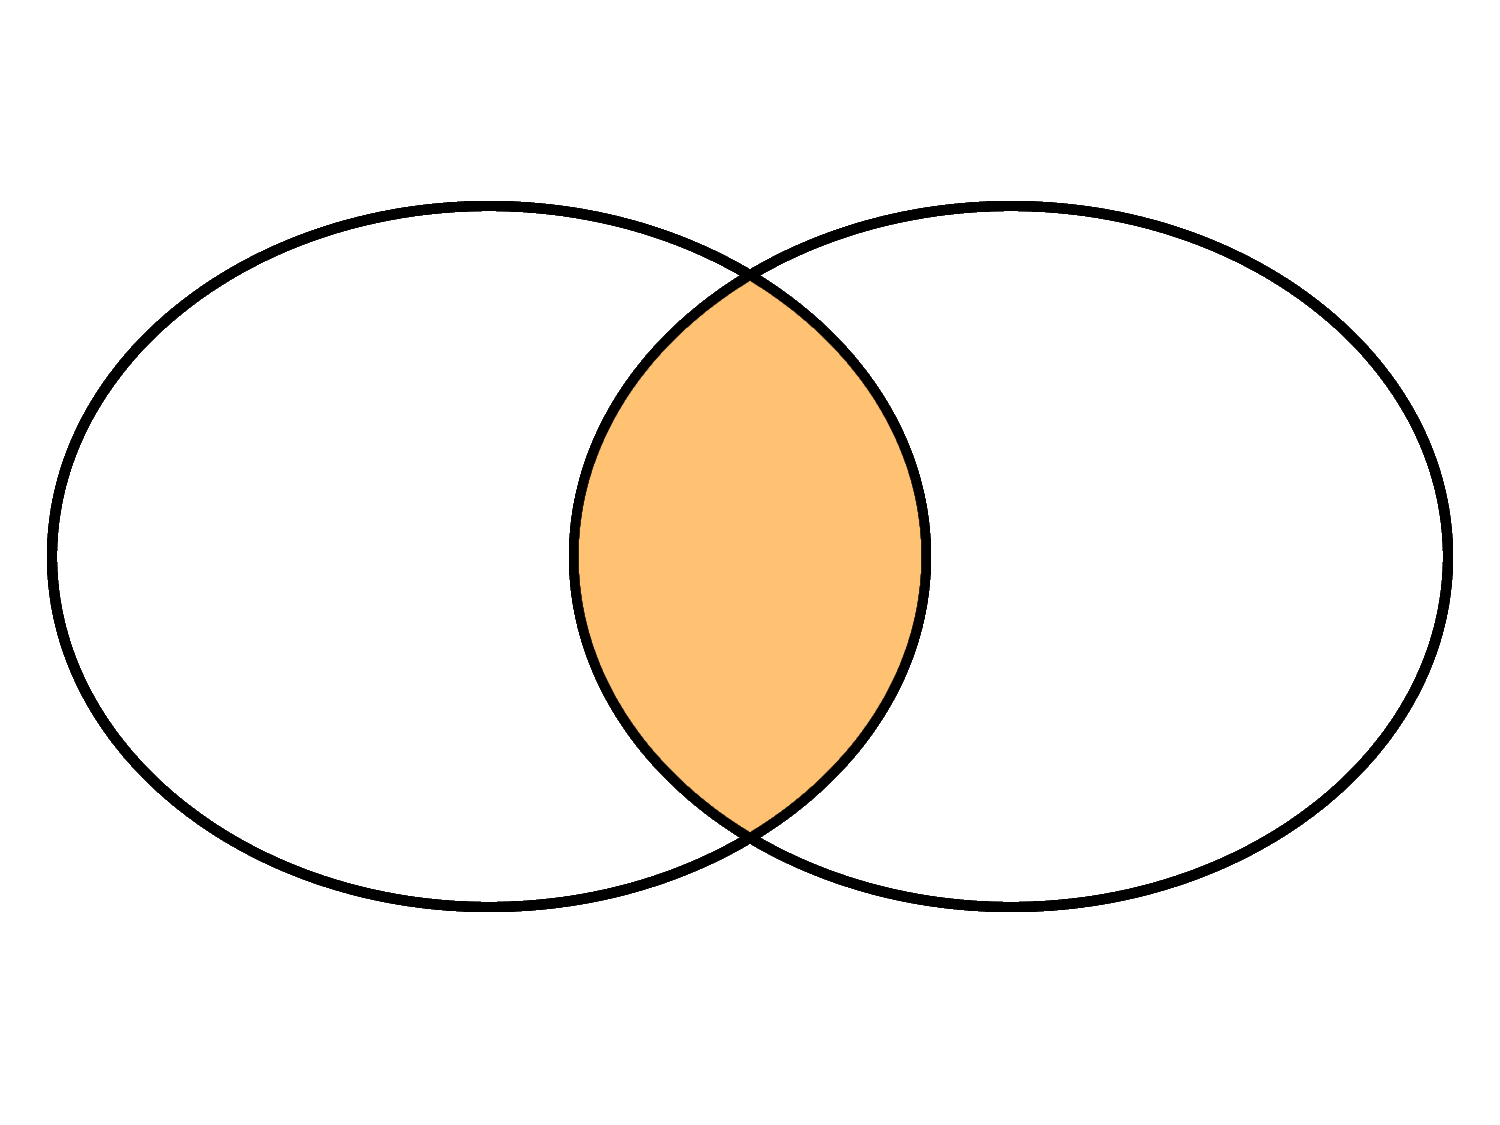
\includegraphics[width=0.7\textwidth]{../figures/AundB.png}
    \caption{Veranschaulichung der Schnittmenge}
    \label{fig:my_label}
\end{figure}
\end{columns}
\end{frame}

\begin{frame}{Mengenoperationen - Vereinigung}
\begin{columns}
\column{0.5\textwidth}
    \begin{alertblock}{Vereinigung - $A\cup B$}
    Gegeben zwei Mengen A und B.\\
    In der Vereinigung liegt alles, das nur in A, nur in B \textbf{oder} in beiden Mengen liegt.
    \end{alertblock}
\column{0.5\textwidth}
\begin{figure}
    \centering
    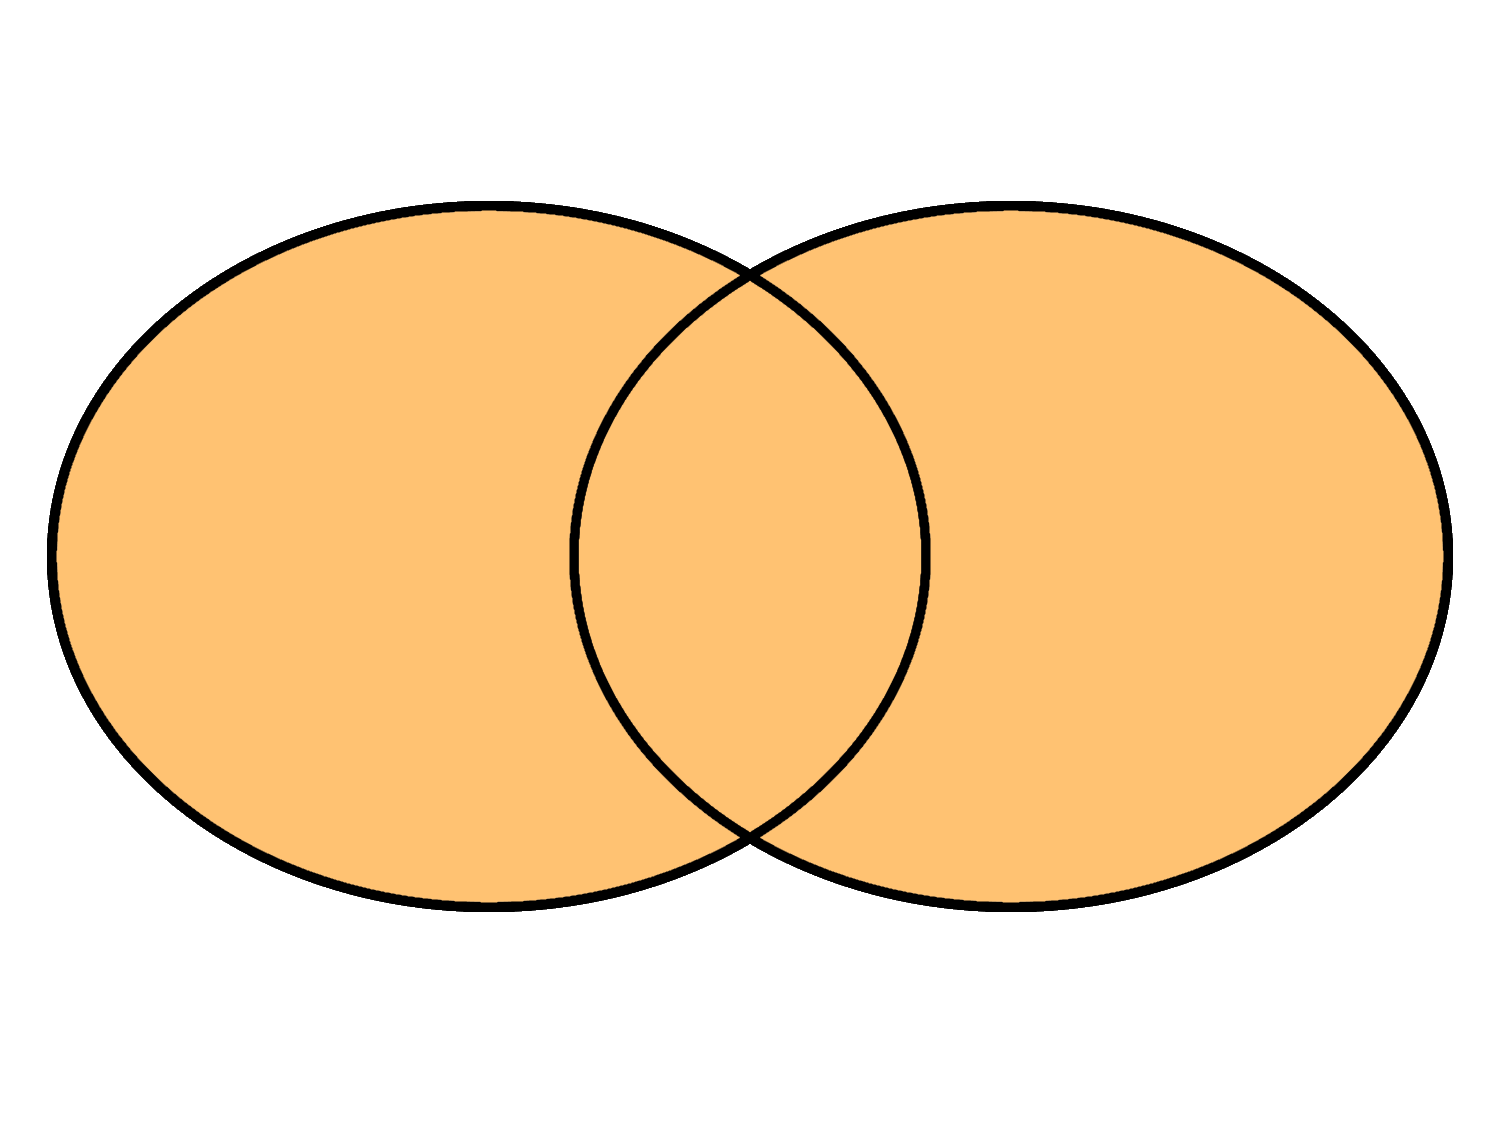
\includegraphics[width=0.7\textwidth]{../figures/AoderB.png}
    \caption{Veranschaulichung der Vereinigung}
    \label{fig:my_label}
\end{figure}
\end{columns}
\end{frame}

\begin{frame}{Mengenoperationen - Komplement}
    \begin{columns}
\column{0.5\textwidth}
    \begin{alertblock}{Komplement - $\overline{A}$}
    Gegeben sei eine Menge A.\\
    Im Komplement der Menge A liegen alle Elemente, die in der Obermenge (z.B. $\Sigma^{*}$), aber nicht in der Menge A selbst liegen.
    \end{alertblock}
\column{0.5\textwidth}
\begin{figure}
    \centering
    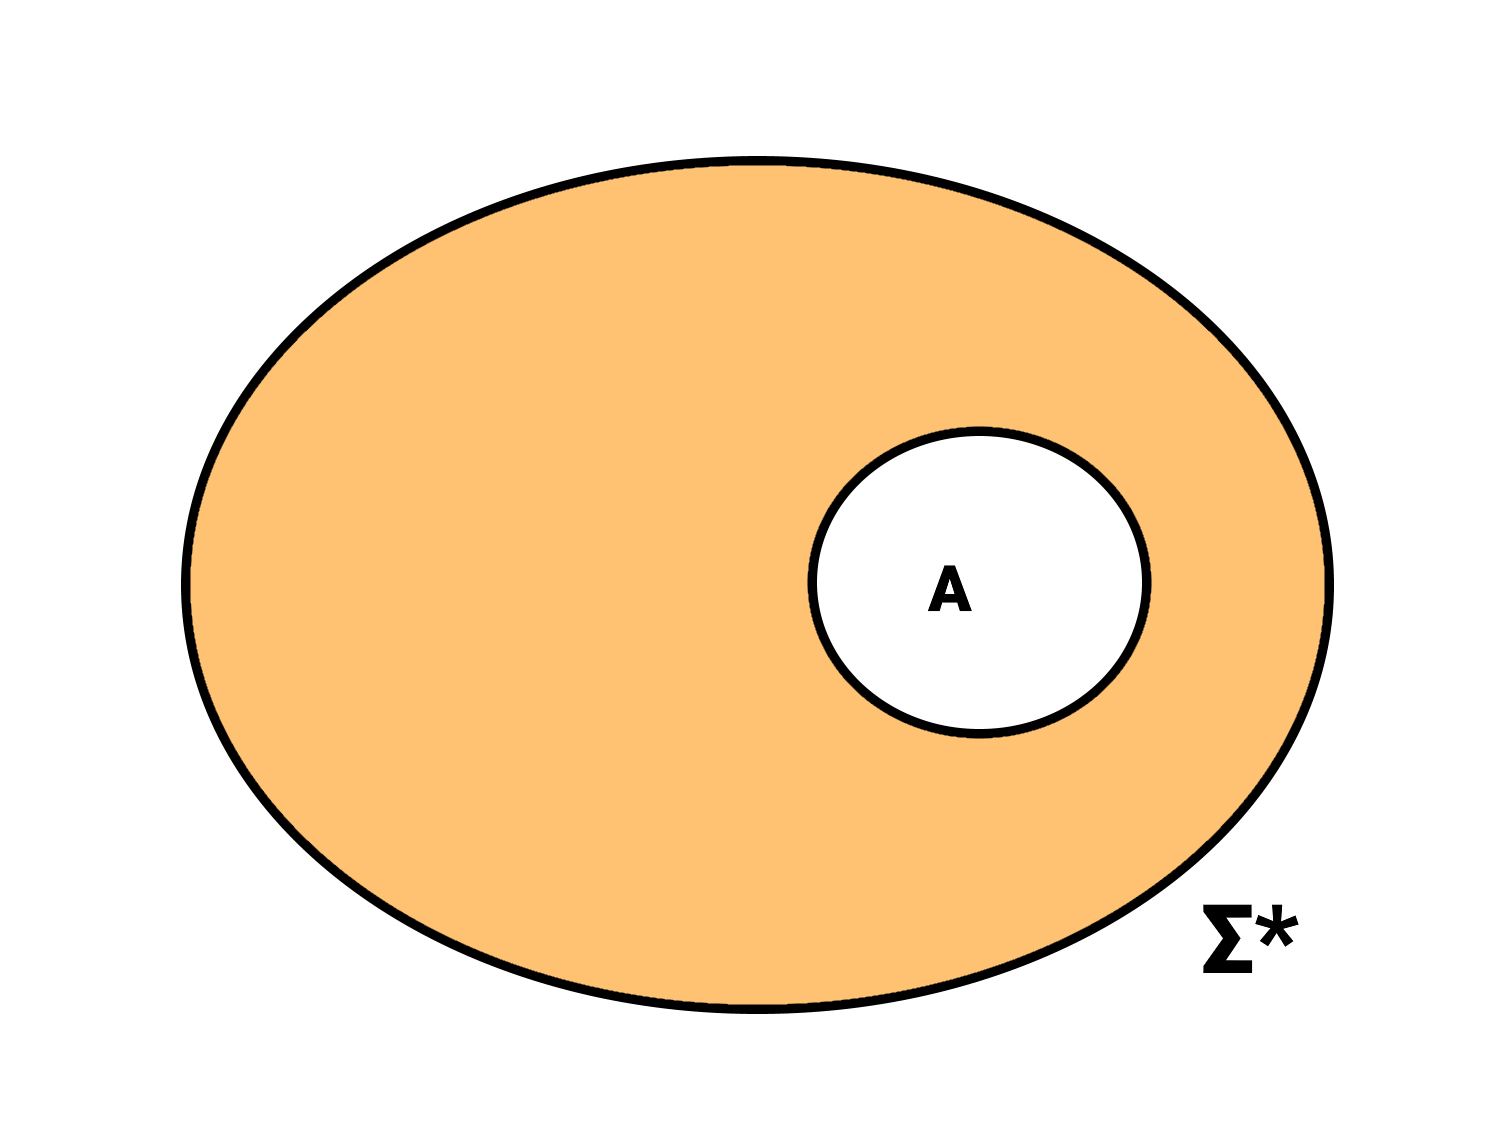
\includegraphics[width=0.7\textwidth]{../figures/Akomp.png}
    \caption{Veranschaulichung des Komplements}
    \label{fig:my_label}
\end{figure}
\end{columns}
\onslide<2>{\alert{\emph{Anmerkung:}} Kann auch geschrieben werden als $\Sigma^{*}\setminus A$. \\
\hspace{2cm}(gesprochen $\Sigma^{*}$ \emph{\glqq ohne\grqq} $A$)}
\end{frame}

\begin{frame}{Mengenoperationen}
    Berechne folgende Mengen
    \metroset{block=fill}
    \begin{alertblock}{Normal}
        \begin{itemize}
            \item $M_1$: $\{a\}\cup \{b\}$
            \item $M_2$: $\{\} \cap \{u, v, w\}$
            \item $M_3$: $\mathbb{N} \cup \mathbb{Z}$
            \item $M_4$: $\overline{\{a^{n}\mid n \ \text{ist gerade}\} }$ , über dem Alphabet $\{a\}$
        \end{itemize}
    \end{alertblock}
        \begin{alertblock}{Schwer bis sehr schwer}
        \begin{itemize}
            \item $M_5$: $\{a, b, c\} \cap  \{a, \{b, c\}\}$
            \item $M_6$: $\{u \mid |u| \equiv 0 \pmod 2, u \in \{a, b\}^{*}\}$\\\hspace{0.65cm}$\cup$ $\{v \mid |v| \equiv 0 \pmod 4, v \in \{a, b\}^{*}\}$
            \item $M_7$: $\overline{\{a^{n} \mid n \ \text{ist gerade}\} }$ , über dem Alphabet $\{a,b\}$
        \end{itemize}
    \end{alertblock}
\end{frame}

{\setbeamercolor{palette primary}{bg=ExColor}
\begin{frame}<handout:0>{Lösungen}
  \begin{itemize}[<+- | alert@+>]
        \item 
            $M_1 = \{a, b\}$
        \item
            $M_2 = \emptyset$
        \item
            $M_3 = \mathbb{Z}$
        \item
            $M_4 = \{a^{n} \mid$ n ist ungerade$\}$ 
        \item
            $M_5 = \{a\}$
        \item
            $M_6 = \{u \mid |u| \equiv 0 \pmod 2, u \in \{a, b\}^{*}\}$
        \item
            $M_7$: $\{a^{n} | n \ \text{ist ungerade}\} \cup\{w | w\in\{a,b\}^{*}, |w|_b \geq 1\}$
    \end{itemize}
\end{frame}
}
